\section{Proof of Determinism for $\lambdaLVar$}\label{section:proof}

\begin{figure*}
%% \rn{I see ``By IH'' is used a lot in the full proof.  But this is the
%%       only occurrence in the paper, and there's enough room on the
%%       line, so let's write out induction hypothesis here?}
\centering
  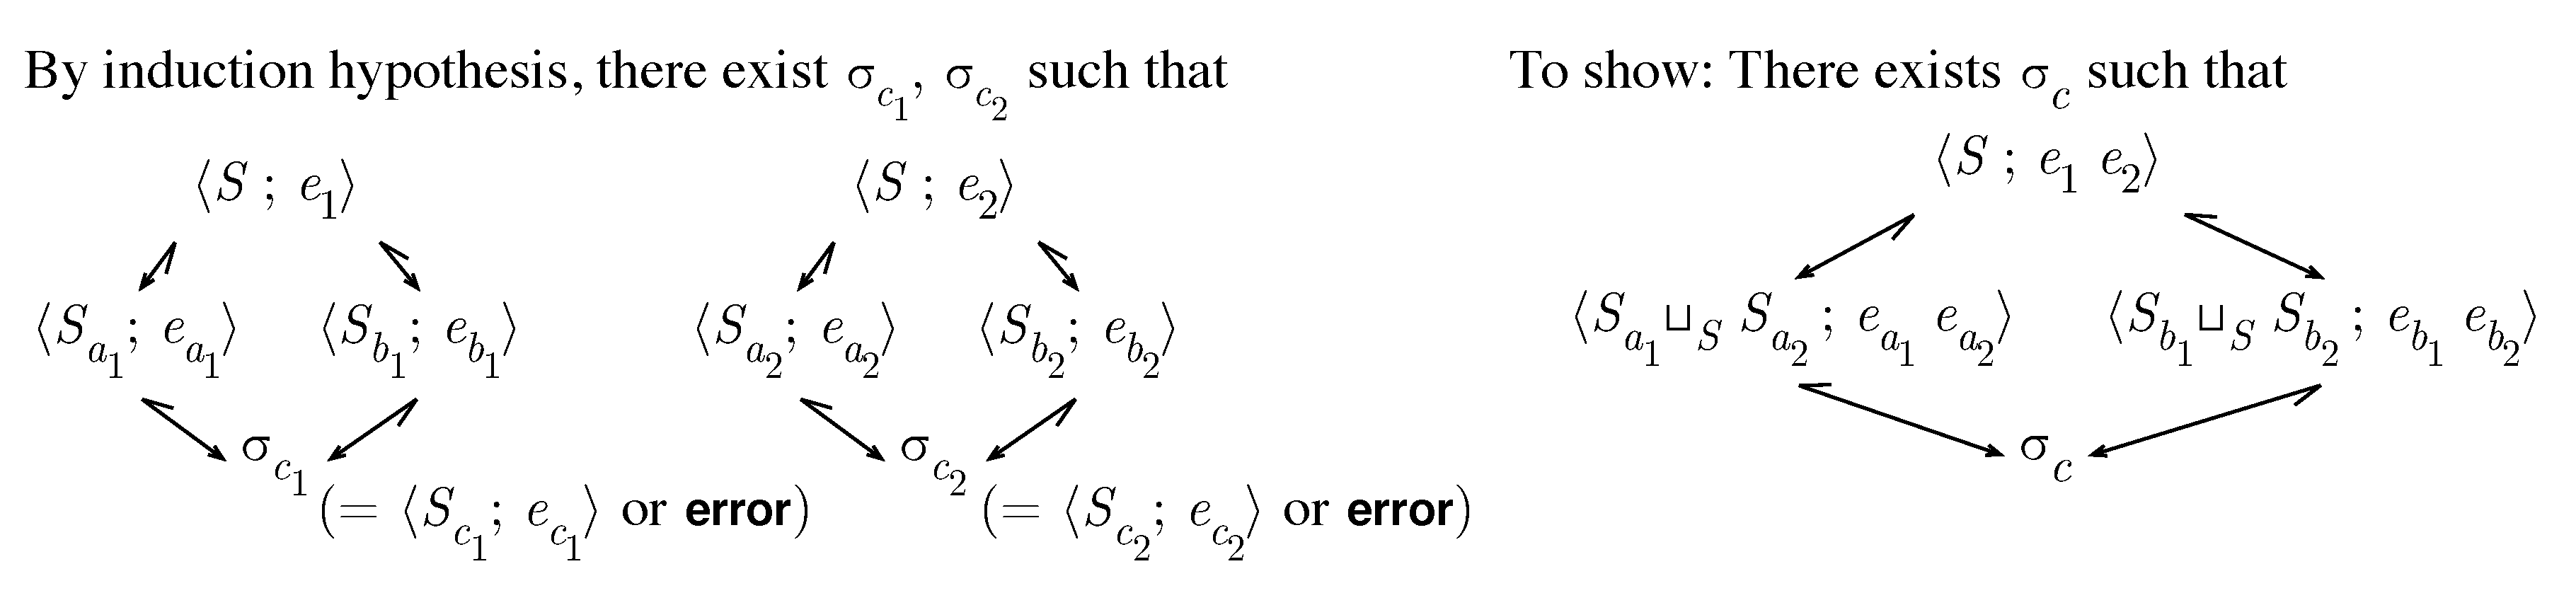
\includegraphics[width=6in,natwidth=1747px,natheight=402px]{chapter2/figures/ParAppParApp.pdf} 
  \caption{\footnotesize Diagram of the subcase of
    Lemma~\ref{lem:diamond}
    in which the {\sc E-ParApp} rule is the last rule in the
    derivation of both $\conf \parstepsto \conf_a$ and $\conf
    \parstepsto \conf_b$.
    We are required to show that, if the
    configuration $\config{S}{\app{e_1}{e_2}}$ steps by {\sc
      E-ParApp} to two different configurations,
    $\config{\lubstore{S_{a_1}}{S_{a_2}}}{\app{e_{a_1}}{e_{a_2}}}$ and
    $\config{\lubstore{S_{b_1}}{S_{b_2}}}{\app{e_{b_1}}{e_{b_2}}}$,
    then they both step to some third configuration $\conf_c$.
  }
  \label{f:diamond-parapp-parapp}
\end{figure*}

Our main technical result is a proof of determinism for the
$\lambdaLVar$ language.
\ifx\fulltr\undefined
%%% Text for paper
Most proofs are only sketched here; the complete
proofs appear in the companion technical
report \cite{lampar-TR}.
\else
%%% Text for TR
The complete proofs appear in Appendix~\ref{app:proof}.
\fi

\subsection{Supporting Lemmas}\label{subsection:independence}

Figure~\ref{f:frame-rule} shows a \emph{frame rule}, due to O'Hearn
\etal~\cite{OHearnLocalReasoning}, which captures the idea that, given
a program $c$ with a precondition $p$ that holds before it runs and
a postcondition $q$ that holds afterward, a disjoint condition $r$
that holds before $c$ runs will continue to hold afterward.
Moreover, the original postcondition $q$ will continue to hold.
For $\lambdaLVar$, we can state and prove an analogous \emph{local reasoning} property.
%% If we think of $c$ as a
%% $\PUT$ operation, and of $p$ and $q$ as, respectively, the state of an
%% LVar before and after the $\PUT$ occurs, then the \emph{local
%%   reasoning} principle we get from such a rule is that we need only
%% worry about the LVar that the $\PUT$ affects, and not the rest of the store
%% (represented by $r$).
\begin{figure}[bt]
    Frame rule (O'Hearn \etal, 2001):
    \begin{mathpar}
      \inferrule*[right=\textnormal{(where no free variable in $r$ is modified by $c$)}]
                 {\lbrace p \rbrace ~ c ~ \lbrace q \rbrace}
                 {\lbrace p * r \rbrace ~ c ~ \lbrace q * r \rbrace}
    \end{mathpar}
    \\
    Lemma~\ref{lem:independence-basic} (Independence), simplified:
    \begin{mathpar}
      \inferrule*[right=\parbox{12em}{\textnormal{($S''$
            non-conflicting with \\
            $\config{S}{e} \parstepsto \config{S'}{e'}$)}}]
      {\config{S}{e} \parstepsto \config{S'}{e'}}
      {\config{\lubstore{S}{S''}}{e} \parstepsto
        \config{\lubstore{S'}{S''}}{e'}}
    \end{mathpar}
  \caption{\footnotesize Comparison of a standard frame rule with a simplified version of
    the Independence lemma.  The $*$ connective in the frame rule requires that its
    arguments be disjoint.  The Independence lemma generalizes $*$ to least upper bound.}
  \label{f:frame-rule}
\end{figure}
Lemma~\ref{lem:independence-basic}, the Independence lemma, says that if the configuration
 $\config{S}{e}$ can step to $\config{S'}{e'}$, then the configuration 
$\config{\lubstore{S}{S''}}{e}$,
where $S''$ is some other store (\eg, one from another subcomputation),
can step to $\config{\lubstore{S'}{S''}}{e'}$.
Roughly speaking, the Independence lemma allows us to ``frame on'' a
larger store around $S$ and still finish the transition with the original result $e'$,
which is key to being able to carry out the determinism proof.

\LemIndependenceBasic

\ifx\fulltr\undefined
\begin{proofsketch}[Proof sketch]
  By induction on the derivation of $\config{S}{e}
  \parstepsto \config{S'}{e'}$, by cases on the last rule in the
  derivation.
\end{proofsketch}
\else
\begin{proof}
See Appendix, Section~\ref{app:independence}.
\end{proof}
\fi

\noindent The Clash lemma, Lemma~\ref{lem:clash-basic}, is similar to the
Independence lemma, but handles the case where $\lubstore{S'}{S''} =
\topS$.  It ensures that in that case, $\config{\lubstore{S}{S''}}{e}$
steps to $\error$.

\LemClashBasic
\ifx\fulltr\undefined
\begin{proofsketch}[Proof sketch]
  By induction on the derivation of $\config{S}{e}
  \parstepsto \config{S'}{e'}$, by cases on the last rule in the
  derivation.
\end{proofsketch}
\else
\begin{proof}
See Appendix, Section~\ref{app:clash}.
\end{proof}
\fi

\noindent Finally, Lemma~\ref{lem:error-preservation} says that if a
configuration $\config{S}{e}$ steps to $\error$, then evaluating $e$
in some larger store will also result in $\error$.

\LemErrorPreservation
\ifx\fulltr\undefined
\begin{proofsketch}[Proof sketch]
  By induction on the derivation of $\config{S}{e}
  \parstepsto \error$, by cases on the last rule in the derivation.
\end{proofsketch}
\else
\begin{proof}
See Appendix, Section~\ref{app:error-pres}.
\end{proof}
\fi

\paragraph{Non-conflicting stores}

In the Independence and Clash lemmas, $S''$ must be \emph{non-conflicting} with
the original transition $\config{S}{e} \parstepsto \config{S'}{e'}$.
We say that a store $S''$ is \emph{non-conflicting} with a
transition $\config{S}{e} \parstepsto \config{S'}{e'}$ iff $\dom{S''}$
does not have any elements in common with $\dom{S'} - \dom{S}$, which
is the set of names of \emph{new} store bindings created between
$\config{S}{e}$ and $\config{S'}{e'}$.

\DefNonConflicting

\noindent The purpose of the non-conflicting requirement is to rule out location
name conflicts caused by allocation.  It is possible to meet
this non-conflicting requirement by applying the $\mathit{rename}$
metafunction, which we define and prove the safety of in
Appendix~\ref{appendix:renaming-lemmas}.

Requiring that a store $S''$ be non-conflicting with a transition
$\config{S}{e} \parstepsto \config{S'}{e'}$ is not as restrictive a
requirement as it appears to be at first glance: it is fine for $S''$
to contain bindings for locations that are bound in $S'$, as long as
they are also locations bound in $S$.  In fact, they may even be
locations that were \emph{updated} in the transition from
$\config{S}{e}$ to $\config{S'}{e'}$, as long as they were not
\emph{created} during that transition.  In other words, given a store $S''$ that is
non-conflicting with $\config{S}{e} \parstepsto \config{S'}{e'}$, it
may still be the case that $\dom{S''}$ has elements in common with
$\dom{S}$, and with the subset of $\dom{S'}$ that is $\dom{S}$.

\subsection{Diamond Lemma}

Lemma~\ref{lem:diamond} does the heavy lifting of our determinism
proof: it establishes the \emph{diamond property}, which says that if a configuration
steps to two different configurations, there exists a single
third configuration to which those configurations both step.
Here, again, we rely on the ability to safely rename locations in a
configuration, as discussed in
Appendix~\ref{appendix:renaming-lemmas}.

\LemDiamond
\ifx\fulltr\undefined
\begin{proofsketch}[Proof sketch]
  By induction on the derivation of $\conf \parstepsto \conf_a$, by
  cases on the last rule in the derivation.
  Renaming is only necessary in the {\sc E-New} case.

  The most interesting
  subcase is that in which the {\sc E-ParApp} rule is the last rule in
  the derivation of both $\conf \parstepsto \conf_a$ and $\conf
  \parstepsto \conf_b$.
  Here, as Figure~\ref{f:diamond-parapp-parapp}
  illustrates, appealing to the induction hypothesis alone is not enough to
  complete the case, and Lemmas~\ref{lem:independence-basic}, 
  \ref{lem:clash-basic}, and \ref{lem:error-preservation} all play a role.  
  For instance, suppose we have from the induction hypothesis that
  $\config{S_{a_1}}{e_{a_1}}$ steps to $\config{S_{c_1}}{e_{c_1}}$.
  To complete the case, we need to show that
  $\config{\lubstore{S_{a_1}}{S_{a_2}}}{\app{e_{a_1}}{e_{a_2}}}$ can
  take a step by the {\sc E-ParApp} rule.
  But for {\sc E-ParApp} to apply,
  we need to show that $e_{a_1}$ can take a step beginning in the
  \emph{larger} store of $\lubstore{S_{a_1}}{S_{a_2}}$.  To do so, we
  can appeal to Lemma~\ref{lem:independence-basic}, which allows us to ``frame
  on'' the additional store $S_{a_2}$ that has resulted from a
  parallel subcomputation.
\end{proofsketch}
\else
\begin{proof}
See Appendix, Section~\ref{app:diamond}.
\end{proof}
\fi

\noindent We can readily restate Lemma~\ref{lem:diamond} as
Corollary~\ref{cor:strong-local-confluence}:

\LemStrongLocalConfluence

%% \rn{With our current version of the semantics, the relation
%%   ${\parstepsto}$ is already ``multi-step'', right?  So do we need
%%   some explanation of what a superscripted ${\parstepsto}^i$ actually
%%   means?  Or is it ok to leave this implicit?}
%% \lk{No, ${\parstepsto}$ is not multi-step; it's parallel, in that it
%%   lets you step two parts of the expression simultaneously, but you
%%   can still only step once.}
\subsection{Confluence Lemmas and Determinism}

With Lemma~\ref{lem:diamond} in place, we can straightforwardly
generalize its result to arbitrary numbers of steps by induction on the number of
steps, as Lemmas~\ref{lem:strong-one-sided-confluence},
\ref{lem:strong-confluence}, and \ref{lem:confluence} show.  
\footnote{Lemmas~\ref{lem:strong-one-sided-confluence},
\ref{lem:strong-confluence}, and \ref{lem:confluence}
  are nearly identical to the corresponding lemmas in
  the proof of determinism for Featherweight CnC given by
  Budimli\'c \etal~\cite{CnC}. We also reuse Budimli\'c \etal's naming
  conventions for Lemmas~\ref{lem:independence-basic} through
  \ref{lem:diamond}, but they
  differ considerably in our setting due to the generality of LVars.}

\LemStrongOneSidedConfluence
\ifx\fulltr\undefined
\begin{proofsketch}[Proof sketch]
  By induction on $m$.  In the base case of $m = 1$, the
  result is immediate from Corollary~\ref{cor:strong-local-confluence}.
\end{proofsketch}
\else
\begin{proof}
See Appendix, Section~\ref{app:strong-one-sided-confluence}.
\end{proof}
\fi

\LemStrongConfluence
\ifx\fulltr\undefined
\begin{proofsketch}[Proof sketch]
  By induction on $n$.  In the base case of $n = 1$, the
  result is immediate from Lemma~\ref{lem:strong-one-sided-confluence}.
\end{proofsketch}
\else
\begin{proof}
See Appendix, Section~\ref{app:strong-confluence}.
\end{proof}
\fi

\LemConfluence

\ThmDeterminism

\subsection{Discussion: Termination}

Above we have followed Budimli\'c \etal~\cite{CnC} in treating {\em
  determinism} separately from the issue of {\em termination}.  Yet
one might legitimately be concerned that in $\lambdaLVar$, a
configuration could have both an infinite reduction path and one that
terminates with a value.  Theorem~\ref{thm:determinism} says that if two runs of a
given $\lambdaLVar$ program reach configurations where no more reductions
are possible (except by reflexive rules), 
then they have reached the same
configuration.  Hence Theorem~\ref{thm:determinism} handles the case of {\em
  deadlocks} already: a $\lambdaLVar$ program can deadlock (\eg, with a blocked $\GET$), but it will do so deterministically.

However, Theorem~\ref{thm:determinism} has nothing to say about {\em
  livelocks}, in which a program reduces infinitely.  It would be
desirable to have a {\em consistent termination} property which
would guarantee that if one run of a given $\lambdaLVar$ program terminates
with a non-$\error$ result,
then every run will.
We
conjecture (but do not prove) that such a consistent termination property
holds for $\lambdaLVar$.
Such a property could be paired with
Theorem~\ref{thm:determinism} to guarantee that if one run of a given
$\lambdaLVar$ program terminates in a non-$\error$ configuration $\sigma$, then every
run of that program terminates in $\sigma$.
(The ``non-$\error$ configuration'' condition is necessary because it
is possible to construct a $\lambdaLVar$ program that can terminate in
$\error$ on some runs and diverge on others.
By contrast, our existing determinism theorem 
%does not require any
%assumptions about fair scheduling, and
does not have to treat $\error$
specially.)

%% Actually, if it's just for non-error configs, then it seems we
%% don't need to assume fair scheduling!

%% , but only if we assume fair
%% scheduling (as is usual when dealing with liveness properties like
%% termination).
%% , and only for programs that do not end in $\error$.  This
%% last condition is necessary because it is possible to construct a $\lambdaLVar$ program that
%% can terminate in $\error$ on some runs and diverge on others.

%% \paragraph{Discussion: Termination}
%% \new{ Above we have followed previous authors \cite{featherweight-cnc} in
%%   treating {\em determinism} separate from the issue of termination.
%%   Yet one might legitimately be concerned that a configuration $\conf$ could
%%   have both an infinite reduction path and one that terminates.  Fortunately, it
%%   turns out that Theorem~\ref{thm:determinism} is in fact strong enough to
%%   prevent this.  We omit the details in this paper, but informally, one can use
%%   determinism to show that a $\lambdaLVar$ creates an isomorphic set of 
%%    $\beta$-reductions in every execution---not just the whole program, but every
%%   expression evaluates to the same value on every execution, only ordering
%%   changes. }

%% \new{A proof by contradiction would assume that a point in the dynamic
%%   evaluation (see {\em pedigree}, Section~\ref{subsection:bump}) returns a
%%   different value in two runs, but that reduction trace is sufficient to
%%   construct a complete program that returns the differing value, violating
%%   \ref{thm:determinism}.  Finally, if every reduction of $\conf$ produces an
%%   isomorphic set of $\beta$-reductions, then it is impossible for one reduction
%%   to diverge (infinite $\beta$-reductions) and another not.  We call this {\em
%%     consistent termination}.}
